%\subsection{Approximate Euler-Maruyama scheme}\label{subsec:euler_maruyama}

\subsection{The sample-based approximate scheme}\label{sec:sample_based}

The update equation \eqref{eq:discretized_noisy_flow} involves computing expectations of the gradient of the kernel $k$ w.r.t the target distribution $\mu$ and the current distribution $\nu_n$ at each iteration $n$. This suggests a simple approximate scheme, based on samples of the two latter distributions, that can be computed in practice. Specifically, we adopt the common approach (sometimes referred to as \textit{mean-field interaction} in mathematical physics and stochastic analysis) which, at each iteration $n$, considers a system of $N$ interacting particles $(X_n^i)_{1\leq i\leq N}$  and their empirical distribution in order to approximate $\nu_n$. 
More precisely, given i.i.d. samples $(X^i_0)_{1\leq i\leq N}$ and $(Y^{m})_{1\leq m\leq M}$ from $\nu_0$ and $\mu$ and a step-size $\gamma$, the approximate scheme iteratively updates the $i$-th particle using: 
\begin{align}\label{eq:euler_maruyama}
X_{n+1}^{i} = X_n^i -\gamma \nabla f_{\hat{\mu},\hat{\nu}_n}(X_n^i+\beta_n U_n^i)
\end{align}
where $U_{n}^{i}$ are i.i.d standard gaussians whereas $\hat{\mu}$ and $\hat{\nu}_n$ denote the empirical distributions of $(Y^{m})_{1\leq m\leq M}$ and $(X^i_n)_{1\leq i\leq N}$. %In \cref{eq:euler_maruyama}, $\nabla f_{\hat{\mu},\hat{\nu}_n}(.)$ can be evaluated easily using only the available samples at iteration $n$:
Implementing \cref{eq:euler_maruyama} is straightforward as it only requires to evaluate the gradient of $k$ on the current particles and target samples.\aknote{add pseudocode}
%\begin{align}
%	 \nabla f_{\hat{\mu},\hat{\nu}_n}(z) = \frac{1}{M}\sum\limits_{m=1}^M \nabla_2 k(Ym,z)-\frac{1}{N}\sum\limits_{j=1}^N \nabla_2 k(X_n^j,z) \qquad \forall z\in\X
%\end{align}
%where $\nabla_2 k(x,z)$ denotes the gradient of $k$ w.r.t. $z$. 
The overall computational cost of such algorithm at each iteration is $O((M+N)N)$ and it uses $O(M+N)$ in memory. The computational cost becomes  $O(M+N)$ when the kernel is approximated using random features as it is the case for regression with neural networks (\cref{subsec:training_neural_networks}). 
This is in contrast to the cubic cost of the flow of the Kernelized Sobolev Discrepancy \cite{Mroueh:2019} which requires solving a linear system at each iteration. This can also be compared to the algorithm in  \cite{csimcsekli2018sliced} which involves computing empirical CDF and quantile functions of random projections of the particles.
The approximation scheme in \cref{eq:euler_maruyama} is a particle version of \cref{eq:discretized_noisy_flow}, so one would expect it to converge towards its population version  \cref{eq:discretized_noisy_flow} as $M$ and $N$ goes to infinity. This is made more formal in the following theorem.
%\begin{theorem}\label{prop:convergence_euler_maruyama}
%Under the same conditions as in \cref{prop:convergence_euler_scheme} and for any $\frac{T}{\gamma}\geq n\geq 0$:
%\begin{equation}
%\mathbb[E][W_2(\hat{\nu}_n,\nu_n)] = \frac{1}{2}(\frac{var(\mu)^\frac{1}{2}}{M} + \frac{(var(\nu_0)^\frac{1}{2})}{N}e^{LT})(e^LT-1)
%\end{equation}
%Where $M(\gamma k)$ is a constant that only depends on $\gamma n$ and the choice of the kernel $k$.
%\end{theorem}
\begin{theorem}\label{prop:convergence_euler_maruyama}
 Let $n\ge 0$ and $T>0$. Let $\nu_n$ and $\hat{\nu}_n$ defined by \eqref{eq:euler_scheme} and \eqref{eq:euler_maruyama} respectively. Suppose \cref{assump:lipschitz_gradient_k} holds and that $\beta_n<B$ for all $n$, for some $B>0$. Then for any $\frac{T}{\gamma}\geq n$:
\[
\mathbb{E}[W_{2}(\hat{\nu}_{n},\nu_{n})]\leq \frac{1}{4}\left(\frac{1}{\sqrt{N}}(B+var(\nu_{0})^{\frac{1}{2}})e^{2LT}+\frac{1}{\sqrt{M}}var(\mu)^{\frac{1}{2}})\right)(e^{4LT}-1)
\]
\end{theorem}
%Notice that since we do not have access to true samples of $\nu_n$ at each iteration $n$, we have adopted the common approach (sometimes referred to as \textit{mean-field interaction} in mathematical physics and stochastic analysis) which considers the system of  $N$ interacting particles $(X_n^{1,N}, X_n^{2,N}, \dots, X_n^{N,N})$ and their empirical distribution in order to approximate $\nu_n$.
\cref{prop:convergence_euler_maruyama} controls the propagation of the chaos at each iteration and uses techniques from \cite{Jourdain:2007}. Notice also that these rates remain true when no noise is added to the updates, i.e. for the original flow when $B=0$. A proof is provided in \cref{proof:propagation_chaos}. The dependence in $\sqrt{M}$ underlines the fact that our algorithm could be interesting as a sampling algorithm when one only has access to $M$ samples of $\mu$ (see \cref{subsec:kl_flow} for a more detailed discussion).

%\begin{remark}
%Two settings are usually encountered in the sampling literature: \textit{density-based}, i.e. the target $\mu$ is known up to a constant, or \textit{sample-based}, i.e. we only have access to a set of samples $X \sim \mu$. The Unadjusted Langevin Algorithm (ULA), which involves a time-discretized version of the Langevin diffusion (see \cref{remark:gradient_flow}), seems much more suitable for first setting, since it only requires the knowledge of $\nabla \log \mu$, whereas our algorithm requires the knowledge of $\mu$ (since $\nabla f_{\mu, \nu_n}$ involves an integration over $\mu$). However, in the sample-based setting, it may be difficult to adapt the ULA algorithm, since it would require firstly to estimate $\nabla \log(\mu)$ based on a set of samples of $\mu$, before plugging this estimate in the update of the algorithm. This problem, sometimes referred to as \textit{score estimation} in the literature, has been the subject of a lot of work but remains hard especially in high dimensions (see \cite{sutherland2017efficient},\cite{li2018gradient},\cite{shi2018spectral}). In contrast, the discretized flow of the $MMD^2$ presented in this section seems naturally adapted to the sample-based setting.
%\end{remark}


%
%
%
%\cref{eq:mcKean_Vlasov_process} suggests a time discretized approximation to \cref{eq:continuity_mmd} which will be analyzed in \cref{sec:convergence_mmd_flow}:
%\begin{align}\cref{eq:time_discretized_flow}
%	X_{n+1} = X_n - \gamma \nabla f_{\nu_n}(X_n) \qquad X_0\sim \nu_0
%\end{align}
%where $\gamma >0$ is the step-size. Using standard techniques from
% 
%
%\paragraph{Modified gradient flow}
%
%
\textbf{Experiments}
%\aknote{if possible get a flat curve for the MMD flow, or precise it's in a log scale/very very slow convergence}

\begin{figure}[ht]
	\centering
	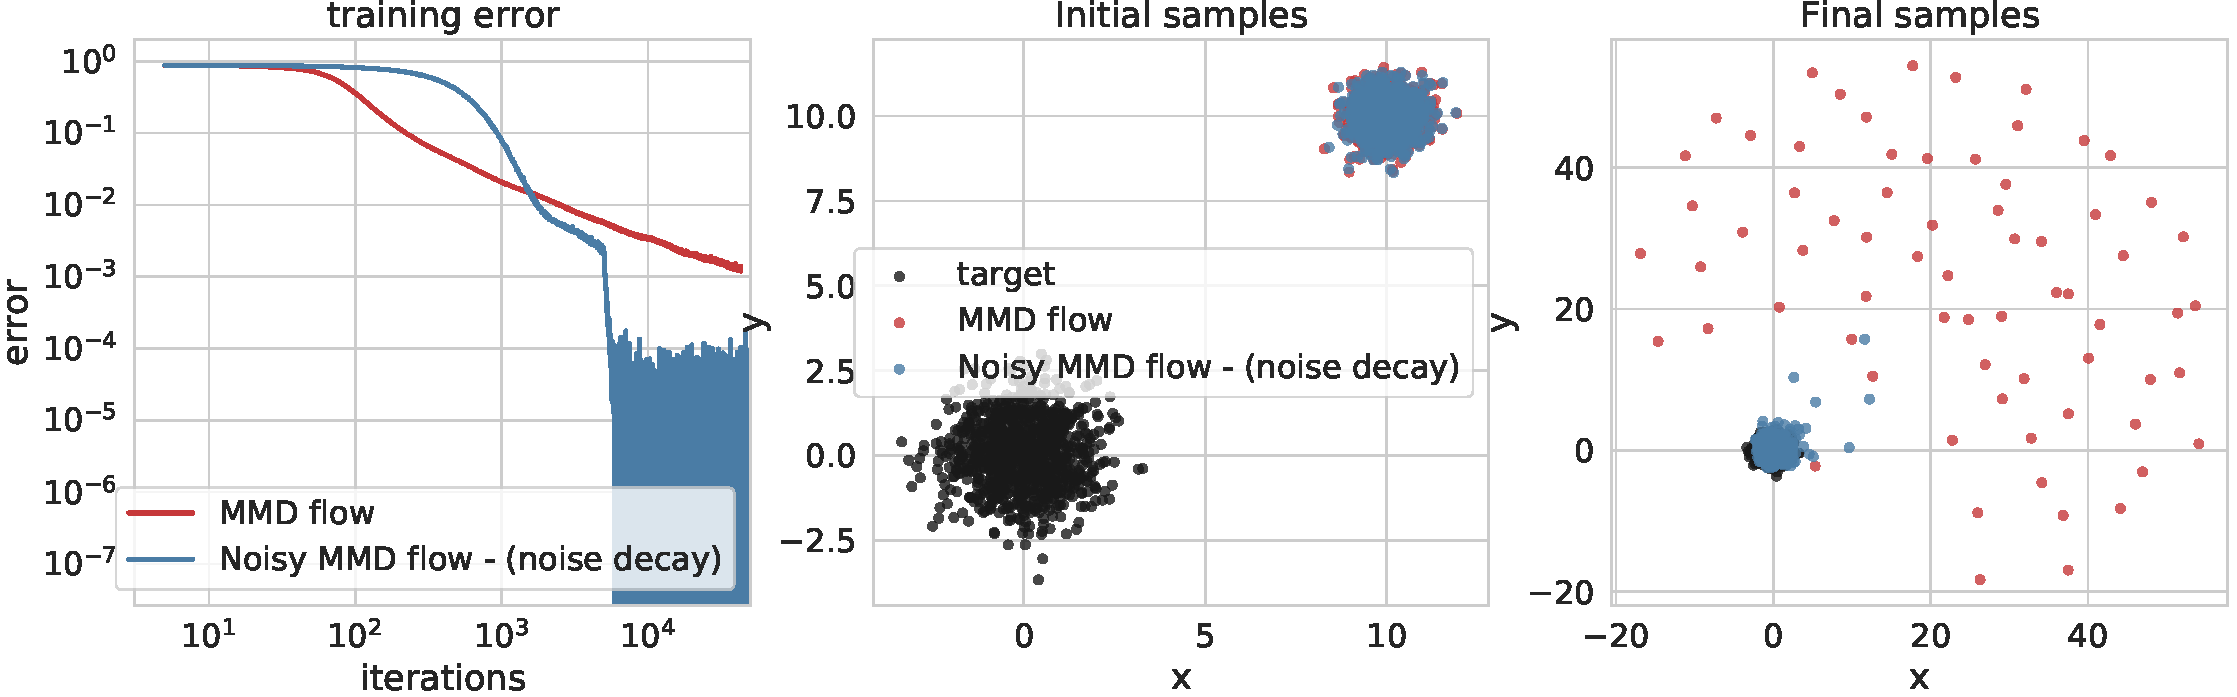
\includegraphics[width=0.8\linewidth]{figures/Gaussians_error_4}
	\caption{Gradient flow of the $MMD$ from a gaussian initial distributions $\nu_0\sim \mathcal{N}(10,0.5)$  towards a target distribution $\mu\sim \mathcal{N}(0,1)$ using $N=M=1000$ samples from $\mu$ and $\nu_0$ and a gaussian kernel with bandwidth $\sigma = 2 $. \cref{eq:euler_maruyama} is used 
	%with noise  $\beta_k = 10$ in blue, 
	without noise $\beta_k = 0$ in red and  with noise $\beta_k = 10$ up to $k=5000$ then $\beta_k = 0$ afterwards in blue. 
	Left figure shows the evolution of the $MMD$ at each iteration. Middle figure shows the initial samples (black for $\mu$) and right figure shows the final samples after $10^5$ iterations with step-size $\gamma = 0.1$.}
	\label{fig:experiments}
\end{figure}
\cref{fig:experiments} illustrates the behavior of the proposed algorithm \cref{eq:euler_maruyama} in a simple setting and compares it with the gradient flow of the MMD without noise injection. In this setting, the MMD flow already fails to converge to the global optimum. Indeed, as shown in \cref{fig:experiments}(right), some of the final samples (in red) obtained using non-noisy gradient updates tend to get further away from the target samples (in black). In fact, most of the remaining samples collapsed to a unique point at the center near the origin. This can also be seen from \cref{fig:experiments}(left) where the training error fails to decrease beyond $10^{-3}$. On the other hand, adding noise to the gradient seems to leads to global convergence as seen visually from the samples. The training error decreases beyond $10^{-4}$ and oscillates between $10^{-8}$ and $10^{-4}$. The oscillation is due to the step-size which remained fixed while the noise was set to $0$ starting form iteration $5000$. It is worth noting that adding noise to the gradient slows the speed of convergence as one can see from \cref{fig:experiments}(left). This is expected since the algorithm doesn't follow the steepest descent. However, the noise helps escaping local optima as  illustrated in this experiment.
